\documentclass[11pt]{article}
\usepackage[T1]{fontenc}
\usepackage[utf8]{inputenc}
\usepackage{lmodern,microtype}
\usepackage[margin=1in]{geometry}
\usepackage{amsmath,amssymb,amsthm,booktabs,longtable,array,graphicx}
\usepackage[colorlinks=true,linkcolor=blue,citecolor=blue,urlcolor=blue]{hyperref}
\hypersetup{pdftitle={A polygon enclosure fails for sums of normal matrices},pdfauthor={Dev D. Goyal},pdfsubject={Exact normal matrices and a straight-segment exterior boundary}}
\newtheorem{theorem}{Theorem}
\title{A polygon enclosure fails for sums of normal matrices}
\author{Dev D. Goyal}
\date{28 October 2026}
\begin{document}
\maketitle
\paragraph{Autonomous AI research disclosure.}
This work is fully autonomous agentic research. Automated systems produced the research, proofs, formalization, and manuscript preparation. Dev D. Goyal is responsible for publication. No expert validation or peer review is claimed.

\begin{abstract}
This note defines a polygon enclosure using segments between permutation values for sums of normal matrices. An explicit pair of normal $3\times3$ matrices gives a determinant outside this region. For spectra $(0,1,i)$ and $(-1-i,1,-1+i)$, a real orthogonal change of basis gives the exact determinant $2/3+2i/9$. The boundary defined by arbitrarily long straight segments that avoid the permutation graph is a simple closed polygon. The determinant lies outside the closure of every bounded component of its complement, and a nonempty bounded component exists. The proof identifies the entire graph, its straight-segment exterior, and a Jordan parametrization. The same determinant is an explicit convex combination of permutation values, so the example respects the ordinary convex-hull inclusion. A companion Lean development verifies the matrix and topological statements. Identification with an external enclosure proposal and historical novelty remain unverified.
\end{abstract}

\begin{theorem}\label{thm:main}
Let $a=(0,1,i)$, $b=(-1-i,1,-1+i)$ and
\[
 U=\frac13\begin{pmatrix}-1&2&2\\2&-1&2\\2&2&-1\end{pmatrix}.
\]
Then $U$ is unitary, $A=\operatorname{diag}(a)$ and $B=U\operatorname{diag}(b)U^*$ are normal, and $\det(A+B)=p=2/3+2i/9$.
The boundary $\Gamma$ of the straight-segment exterior of their full transposition graph is the Jordan polygon with consecutive vertices
\[
 6-2i,\quad2+i,\quad2i,\quad1,\quad-i,\quad2-2i.
\]
There is a nonempty bounded connected component of $\mathbb C\setminus\Gamma$, and $p$ lies outside the closure of every bounded connected component. Nevertheless, $p$ lies in the convex hull of the six permutation values.
\end{theorem}

The definitions and proof follow. The gap is visible at height $2/9$: the left boundary has real coordinate $8/9$, while $\operatorname{Re}p=2/3$. The argument must also identify that polygon as the boundary specified by the straight-segment exterior; choosing a cycle in the graph alone would not suffice.

\section{The precise problem}\label{the-precise-problem}

For two lists of complex eigenvalues \(a=(a_1,\ldots,a_n)\) and
\(b=(b_1,\ldots,b_n)\), write

\[
D_a=\operatorname{diag}(a_1,\ldots,a_n),\qquad
D_b=\operatorname{diag}(b_1,\ldots,b_n),
\]

and define their determinant range

\[
\Delta(a,b)=\{\det(D_a+UD_bU^*):U\text{ is unitary}\}.
\]

The permutation points are

\[
z_\sigma=\prod_{j=1}^n(a_j+b_{\sigma(j)}),\qquad \sigma\in S_n.
\]

The motivating enclosure proposal is attributed to
Kova\v{c}ec~\cite{kovacec2026}. Its literal Definition 6, Conjecture 7,
and current-version hypotheses have not been verified here. The following
definitions are the exact model proved in this note. An external
refutation is conditional on agreement with these definitions and
quantifiers.

Draw a segment between two permutation points when the corresponding
permutations differ by one transposition. Let \(G\) be the union of
these segments. Call a point exterior if, for every \(M>0\), a straight
segment of length \(M\) starting there avoids all edges of \(G\).
This is a visibility condition, distinct from an arbitrary path to infinity.

In formulas, for the closed real segment $[z,w]=\{(1-t)z+tw:0\le t\le1\}$, the exterior is
\[
 E(G)=\{z:\forall M>0\ \exists w,\ |w-z|=M\ \text{and}\ [z,w]\cap G=\varnothing\}.
\]
The direction is permitted to depend on $M$. Write $\Gamma=\partial E(G)$.

The enclosure tested here places \(\Delta(a,b)\) in the closure of a
bounded complementary component when this boundary is a Jordan curve.
The construction below violates this standalone enclosure, with the
Jordan hypothesis verified for the specified spectra.

\section{Exact normal matrices}\label{exact-normal-matrices}

Take

\[
a=(0,1,i),\qquad b=(-1-i,1,-1+i),
\]

and

\[
U=\frac13
\begin{pmatrix}
-1&2&2\\
2&-1&2\\
2&2&-1
\end{pmatrix}.
\]

Let \(\mathbf{J}\) denote the three-by-three all-ones matrix. Then
\(U=(2\mathbf J-3I)/3\), and \(\mathbf J^2=3\mathbf J\). Hence

\[
U^2=I,\qquad U^{\mathsf T}=U,
\]

so \(U\) is real orthogonal and therefore complex unitary. Define
\(A=D_a\) and \(B=UD_bU^*\). Both matrices are normal and have the
required unitary spectral representations. Explicitly,

\[
B=\frac19
\begin{pmatrix}
-1+3i&-4+6i&8\\
-4+6i&-7&-4-6i\\
8&-4-6i&-1-3i
\end{pmatrix}.
\]

The sum is

\[
A+B=\frac19
\begin{pmatrix}
-1+3i&-4+6i&8\\
-4+6i&2&-4-6i\\
8&-4-6i&-1+6i
\end{pmatrix},
\]

and direct determinant expansion gives

\[
\det(A+B)=\frac{486+162i}{729}=\frac23+\frac29 i=p.
\]

For example, set $\alpha=-1+3i$, $\beta=-4+6i$, $\gamma=-4-6i$ and $\delta=-1+6i$. Expansion of the numerator matrix along its first row gives
\begin{align*}
 9^3\det(A+B)&=\alpha(2\delta-\gamma^2)-\beta(\beta\delta-8\gamma)+8(\beta\gamma-16)\\
 &=\alpha(18-36i)-\beta(18i)+288\\
 &=(90+90i)+(108+72i)+288=486+162i.
\end{align*}
All quantities here are exact. No numerical eigenvalue calculation or floating-point tolerance enters the proof.

\section{The permutation graph}\label{the-permutation-graph}

Number the six permutations lexicographically, beginning at zero:

\begin{longtable}[]{@{}rcl@{}}
\toprule\noalign{}
Index & Permutation & Permutation point \\
\midrule\noalign{}
\endhead
\bottomrule\noalign{}
\endlastfoot
0 & 123 & \(v_0=6-2i\) \\
1 & 132 & \(v_1=2\) \\
2 & 213 & \(v_2=2+i\) \\
3 & 231 & \(v_3=-i\) \\
4 & 312 & \(v_4=2i\) \\
5 & 321 & \(v_5=2-2i\) \\
\end{longtable}

The complete list of unordered transposition edges is

\[
01,\ 02,\ 05,\ 13,\ 14,\ 23,\ 24,\ 35,\ 45.
\]

Each permutation has three transposition neighbors. Their index lists are, in order, $(1,2,5)$, $(0,3,4)$, $(0,3,4)$, $(1,2,5)$, $(1,2,5)$ and $(0,3,4)$. This exhausts the three transpositions at every permutation and yields exactly the nine unordered edges above.

The segments \([v_2,v_3]\) and \([v_4,v_5]\) intersect at

\[
w=1.
\]

Let \(C\) be the closed polygon whose vertices, in cyclic order, are

\[
(6,-2),\quad(2,1),\quad(0,2),\quad(1,0),\quad(0,-1),\quad(2,-2).
\]

Every boundary segment belongs to the permutation graph: the successive
sides are pieces of edges \(02,24,45,23,35,05\). Every graph edge lies
in \(C\).

\begin{figure}[tb]
\centering
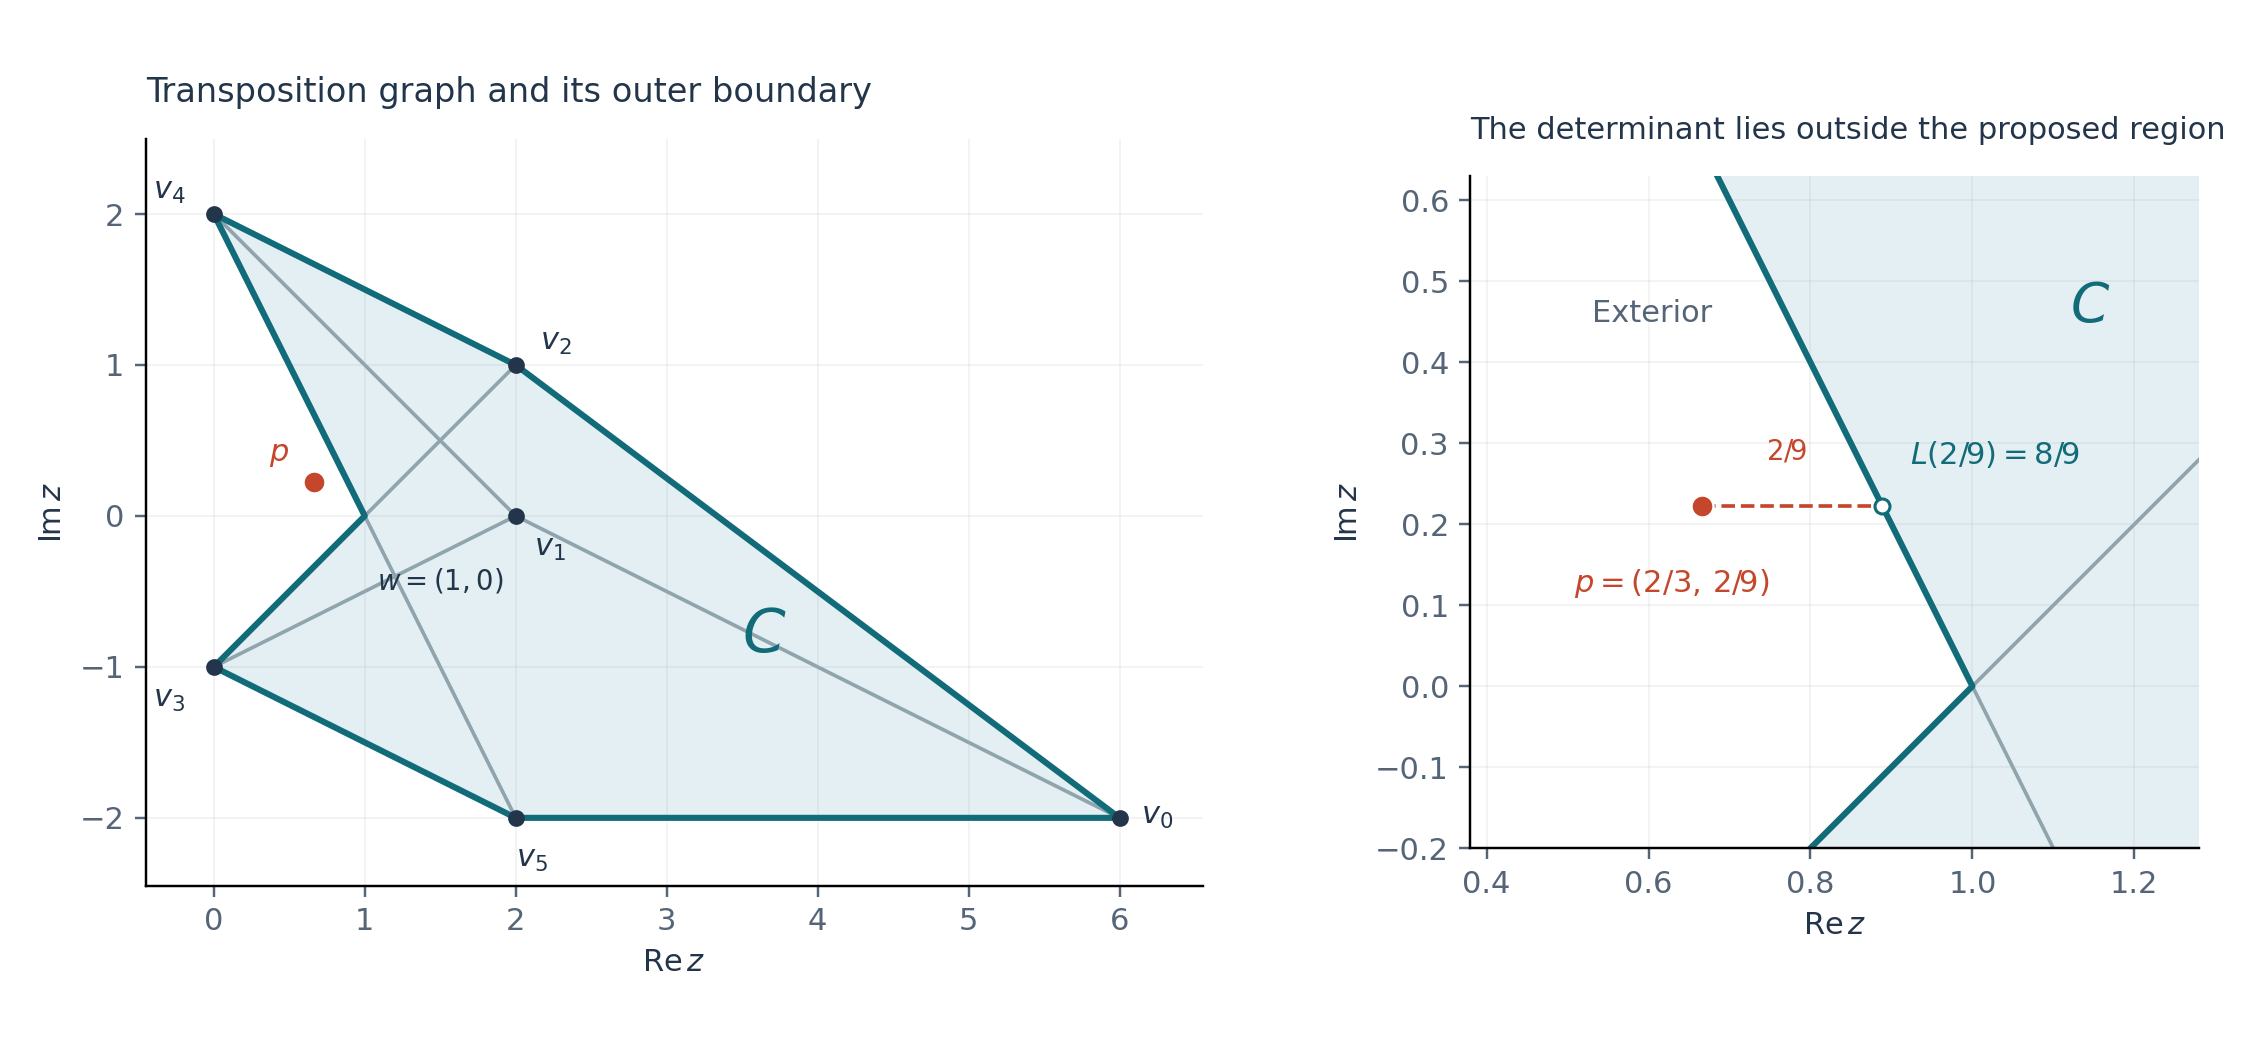
\includegraphics[width=\linewidth]{figures/kovacec_counterexample.png}
\caption{The complete transposition graph and its exterior boundary (left), with the indentation at $w=1$ enlarged (right). The determinant $p$ is a horizontal distance $2/9$ to the left of the polygon at height $2/9$. The exact formulas, rather than measurements from this drawing, prove the separation.}
\end{figure}

\section{Exact identification of the exterior and the Jordan boundary}\label{exact-identification-of-the-exterior-and-the-jordan-boundary}

The horizontal section of \(C\) at height \(y\) is

\[
C\cap\{\operatorname{Im}z=y\}
=\{x+iy:L(y)\le x\le R(y)\},\qquad -2\le y\le2,
\]

and is empty outside that height interval. The boundary functions are

\[
L(y)=
\begin{cases}
-2y-2,&-2\le y\le-1,\\
y+1,&-1\le y\le0,\\
1-y/2,&0\le y\le2,
\end{cases}
\]

and

\[
R(y)=
\begin{cases}
(10-4y)/3,&-2\le y\le1,\\
4-2y,&1\le y\le2.
\end{cases}
\]

The functions are continuous, and $R-L$ is affine on the intervals cut out by heights $-2,-1,0,1,2$. Its values at those heights are $4,14/3,7/3,3/2,0$, respectively. Hence $L<R$ below height $2$, while $L(2)=R(2)=0$. The set $C$ is closed and bounded. Its interior is exactly
\[
 \{x+iy:-2<y<2,\ L(y)<x<R(y)\}.
\]
Strict inequalities give interior points by continuity. Equality in either horizontal bound permits an arbitrarily small horizontal move outside $C$, and an extreme height permits a vertical move outside $C$. Thus the boundary is exactly the two graphs $x=L(y)$ and $x=R(y)$ on $[-2,2]$, joined by the bottom segment $[2-2i,6-2i]$.

For completeness, every nonhorizontal graph edge has the following equation. The indicated height interval includes both endpoints.
\begin{center}
\begin{tabular}{@{}ccc@{}}
\toprule Edge & Height interval & Real coordinate $x(y)$\\\midrule
01&$[-2,0]$&$2-2y$\\
02&$[-2,1]$&$(10-4y)/3$\\
13&$[-1,0]$&$2y+2$\\
14&$[0,2]$&$2-y$\\
23&$[-1,1]$&$y+1$\\
24&$[1,2]$&$4-2y$\\
35&$[-2,-1]$&$-2y-2$\\
45&$[-2,2]$&$1-y/2$\\\bottomrule
\end{tabular}
\end{center}
For each row, $L(y)\le x(y)\le R(y)$ on its interval: split at $-1,0,1$ and check the endpoint inequalities, since every difference is affine on each piece. The remaining edge $05$ has $y=-2$ and $2\le x\le6$. This proves that the entire graph lies in $C$. Conversely, the right boundary consists of edges $02$ and $24$. The left boundary consists of edge $35$, the part of edge $23$ from $-i$ to $1$, and the part of edge $45$ from $1$ to $2i$. Together with edge $05$, these give the entire boundary. Hence $\partial C$ lies in the graph.

For an explicit Jordan certificate, parameterize the six sides over
\([0,6]\):

\[
q(t)=
\begin{cases}
(6-4t)+i(-2+3t),&0\le t\le1,\\
(4-2t)+it,&1\le t\le2,\\
(t-2)+i(6-2t),&2\le t\le3,\\
(4-t)+i(3-t),&3\le t\le4,\\
(2t-8)+i(3-t),&4\le t\le5,\\
(4t-18)-2i,&5\le t\le6.
\end{cases}
\]

The formulas agree at every joining point, so $q$ is continuous and $q(0)=q(6)=6-2i$. On $[0,2]$, the path follows the right graph $x=R(y)$ with height strictly increasing from $-2$ to $2$. On $[2,5]$, it follows the left graph $x=L(y)$ with height strictly decreasing from $2$ to $-2$. Since $L<R$ below the top, these arcs meet only at their common top endpoint. On $[5,6]$, the bottom path has height $-2$ and real coordinate strictly increasing from $2$ to $6$; it meets the other arcs only at its endpoints. Thus $q$ is injective on $[0,6)$. The boundary description above shows that its image is precisely $\partial C$. This proves the Jordan condition directly.

The next step verifies the displayed exterior convention. Every point outside
\(C\) has a straight escape ray. At heights between \(-2\) and \(2\), a
point to the left of \(L(y)\) escapes horizontally left, and a point to
the right of \(R(y)\) escapes horizontally right. Points above or below
the polygon escape vertically. Since the graph lies in \(C\), these rays
avoid every edge.

Conversely, a point on \(\partial C\) belongs to the graph, so a segment
starting there already intersects the graph. A point in the interior of
\(C\) cannot have an arbitrarily long graph-avoiding segment:
choose a length $M$ greater than the diameter of the compact set $C$. Every endpoint at distance $M$ from the interior point is outside $C$. A segment joining the two points must meet $\partial C$: otherwise its connected image would meet both of the disjoint open sets $\operatorname{int}C$ and $\mathbb C\setminus C$ while lying in their union. Since $\partial C$ is contained in the graph, no such segment avoids the graph.

Consequently the displayed exterior is \textbf{exactly}
\(\mathbb C\setminus C\), and its boundary is the verified Jordan curve
\(\partial C\).

\section{Failure of the defined enclosure}\label{failure-of-the-defined-enclosure}

At the determinant's height,

\[
\operatorname{Im}p=\frac29,\qquad
L\!\left(\frac29\right)=\frac89,
\]

whereas

\[
\operatorname{Re}p=\frac23<\frac89.
\]

Thus \(p\notin C\), with an exact horizontal gap of \(2/9\) from the
left boundary. Its entire left horizontal ray stays outside \(C\), and
hence outside the permutation graph.

For completeness, the formal proof also addresses the bounded
complementary component directly. Every point outside \(C\) has an
unbounded connected escape ray lying outside its frontier. The connected
component of \((\partial C)^c\) containing that point is therefore
unbounded. It follows that every bounded connected component of
\((\partial C)^c\) lies inside \(C\); since \(C\) is closed, its closure
also lies in \(C\). Therefore

\[
p\notin\overline K
\quad\text{for every bounded connected component }K
\text{ of }(\partial C)^c.
\]

There is a bounded nonempty component: \(2+0i\) is an interior point
because

\[
-2<0<2,\qquad L(0)=1<2<R(0)=\frac{10}{3}.
\]

The complement of the frontier is the disjoint union of the open sets $\operatorname{int}C$ and $\mathbb C\setminus C$. Its connected component containing $2$ meets the first, so connectedness prevents it from meeting the second. The component is therefore nonempty and contained in the bounded set $C$. The counterexample consequently satisfies the displayed
existence and Jordan hypotheses, and defeats every possible
bounded-component enclosure. No unproved general Jordan curve theorem or
uniqueness assertion is used in the formal proof.

This proves failure of the stated polygon enclosure, with all of its geometric hypotheses satisfied.

\section{Why this does not contradict the classical conjecture}\label{why-this-does-not-contradict-the-classical-conjecture}

The determinant has the explicit convex representation

\[
p=\frac19v_0+\frac49v_3+\frac49v_4.
\]

The three weights are nonnegative and sum to one. Thus \(p\) belongs to
the ordinary convex hull of the permutation points. The three points
used here correspond to the even permutations \(123,231,312\); no pair
of them is joined by a single-transposition edge. Their convex
combinations need not stay within the smaller polygon defined here.

The exact identity is checked by the following Lean declaration:

\begin{verbatim}
KovacecResolution.ordinary_convex_combination
\end{verbatim}


\section{Formal verification and scope}
The proof above establishes Theorem~\ref{thm:main} without a computer calculation. Its formal counterpart consists of eight proof modules and a root import file. The matrix certificate verifies the actual matrices, unitarity, normality, determinant, all six permutations and all nine transposition edges. The geometric modules define the boundary functions, prove the exact frontier and loop image, and verify injectivity. The exterior and component modules prove equality with the straight-segment exterior and exclusion from all bounded component closures.

The endpoint \texttt{KovacecResolution.completed\_counterexample} includes the two normality identities, exact determinant, Jordan condition, existence of a nonempty bounded component, and exclusion from every bounded component closure. The package-defined predicate \texttt{Conjecture7} asks for a bounded component closure containing the determinant under the displayed hypotheses. The theorem \texttt{conjecture7\_false} refutes that formal predicate. These names do not authenticate an external Conjecture 7 or its definitions. No general Jordan-curve uniqueness theorem is needed. The separate theorem \texttt{ordinary\_convex\_combination} verifies the convex identity.

The checked endpoint dependencies are exactly \texttt{propext}, \texttt{Classical.choice} and \texttt{Quot.sound}. The formalization map identifies the declarations and reproduction commands. Formal verification checks these stated objects and assumptions; it does not establish novelty, external source identity, or publication priority.

The result concerns the stated polygon enclosure. It does not refute the Marcus--de Oliveira convex-hull conjecture or resolve that conjecture in general. Its scope is an exact obstruction in dimension three, with a real orthogonal mixing matrix and the full geometric hypotheses verified.

\bibliographystyle{plain}
\bibliography{references}
\end{document}
